\chapter{Hellman}
%%% Local Variables:
%%% mode: latex
%%% TeX-master: "Thesis"
%%% End:
Hellman tradeof is the first iteration of time memory trade offs, It was first explained in the paper A Cryptanalytic Time - Memory Trade-Off by Martin Hellman.
The idea is similar to a naive table lookup where all possible keys K have been encrypted with the plaintext P. Instead of storing all the key ciphertext pairs which is done in the naive table lookup all pairs are sorted into several chains where the only part stored is the start point and the end point. This way memory is saved but time is increased for the online phase. To find a pair one needs to find the right chain and look up the pair.


\subsection*{Precomputation phase}
Like any other tmto the table itself is generated in the precomputational phase. Each table is fixed for a single plaintext.
The Helman tradof has 3 main parameters, m, t and l and they decide the size of the table that will be generated.
m is the amount of rows, t is the columns, and l is the amount of times they are repeated.
Certain requirements are put on these parameters, The size of m*t*t must not be much larger or much smaller than N.
N is the keysize of the cipher we are trying to break. We use a Matrix stopping constant (Hmsc) to hold the difference between N and m*t*t. Hmsc can therefore not be very large nor very close to zero.

##add om reduction function

By selecting the parameters the table can be generated. This is done by selecting m random starting points, $ sp^{k}_1,sp^{k}_2,...,sp^{k}_m E N$. Each startingpoint is then used as the start of their chain and with recursion the chain links are computed by $ x^{k}_{i,j}=F_k( x^{k}_{i,j-1})$ for $0<j<=t$. When the endpoint is reached it is stored as a pair with the startpoint ${( sp^{k}_{i}, ep^{k}_{i})}^{m}_{i=1}$.
The Hellman table/matrix is usually visualized like so:
\\sad
\begin{figure}[t]
  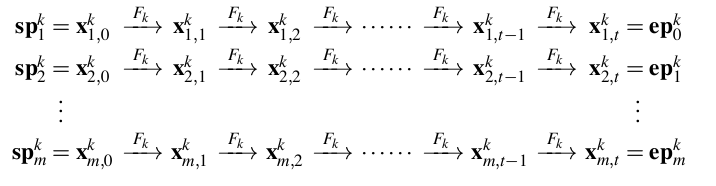
\includegraphics[width=8cm]{figures/HellmanMatrix.png}
\centering
\end{figure}
\subsection*{Online phase}
\subsection*{Analasys}
